\documentclass[runningheads,a4paper]{llncs}

\usepackage{amssymb}
\setcounter{tocdepth}{3}
\usepackage{graphicx}
\usepackage{amsmath}
\usepackage{verbatim}
\usepackage[margin=0.9in]{geometry}
%\usepackage{amsfonts}
%\usepackage{amsthm}
\usepackage{subfigure}
\usepackage{mathtools}
%\usepackage{caption}
%\usepackage{subcaption}
%\usepackage{cite}
\usepackage{hyperref}
\usepackage{url}
\urlstyle{same}
\newcommand{\keywords}[1]{\par\addvspace\baselineskip
\noindent\keywordname\enspace\ignorespaces#1}

\makeatletter
\let\c@lemma=\c@theorem
\let\c@corollary=\c@theorem
\let\c@fact=\c@theorem
\makeatother

\let\realendproof=\endproof
\def\endproof{\hspace*{\fill}$\Box$\realendproof}


\begin{document}

\title{Poker Chips, Earthquakes, and Computation}
\titlerunning{Poker Chips, Earthquakes, and Computation}

\author{Perry Kleinhenz \and Fermi Ma \and Erik Waingarten}
%
\authorrunning{Perry Kleinhenz \and Fermi Ma \and Erik Waingarten}
% (feature abused for this document to repeat the title also on left hand pages)

% the affiliations are given next; don't give your e-mail address
% unless you accept that it will be published
\institute{
\protect\url{{pkleinhe, fermima,eaw}@mit.edu}}

\maketitle

\section{Introduction}

\emph{Written by Fermi Ma, edited by Erik Waingarten and Perry Kleinhenz.}\\

\noindent In this paper, we investigate the following problem:

\vbox{
\noindent
\begin{quote}
Each node of an infinite grid graph contains some nonnegative number of chips. An earthquake hits one node that has at least four chips and redistributes them so that one chip moves to each of its four neighbors.
\end{quote}
}

In Section~\ref{Definitions and Notation}, we formalize the terminology and operations we use to analyze the problem. In particular, we formalize the effects of earthquakes, as well as what it means for a board of chips to be finite or infinite. 
In Section~\ref{Stability of Finite Boards}, we introduce a spread function that maps finite board configurations to $\mathbb{R}$. 
We then use the fact that earthquakes strictly increase the value of this spread function to show that finite boards cannot cycle back to previous configurations, from which we will conclude that all finite boards reach a steady state. Then we show that this means that no boards can return to their same state. 
From this, we conclude that such boards never cycle back to previous configurations. 
In Section~\ref{Order of Redistribution}, we show that for a given board the number of times a particular square must be hit by a earthquake in order for a board to stabilize is independent of the order in which the earthquakes occur. 

For the remainder of the paper, we consider other approaches and extensions of the problem. 
In  Section~\ref{Time until Stability}, we present results from our computer simulations of repeated earthquakes. In particular, we look at the starting arrangement where all of the board's $n$ chips are initially on one central square.
We conjecture based on experimental evidence that such arrangements stabilize after $\Theta(n \log n)$ global earthquakes. 
In Section~\ref{Board Variants: d-Trees}, we generalize away from the infinite grid graph and consider what happens when a similar process happens on tree graphs of infinite size. 
Finally, in Section~\ref{Computing with Chips} we present a model of computation based on the poker chip board and show how to construct simple Boolean circuits. We will also give impossibility results that show the limits of our model of computation.
\section{Definitions and Notation}
\label{Definitions and Notation}

\emph{Written by Erik Waingarten, edited by Fermi Ma and Perry Kleinhenz.}\\

First, we formalize the board of poker chips. We consider the integer lattice $\mathbb{Z} \times \mathbb{Z}$ as the set of nodes, indexed by the corresponding coordinate. We made the two nodes have an edge between them if they are a distance of 1 apart.

\begin{definition} A board is a function $b: \mathbb{Z} \times \mathbb{Z} \to \mathbb{Z}_{\geq 0}$.
The input to this function correspond to the nodes and the output is the number of chips on that node. Let $\mathcal{B}$ denote the set of all boards.
\end{definition}

In order to keep our notation compact we let $n(i,j)$ be the set of neighbors of node $(i,j)$.
\begin{definition}
We define the function $n: \mathbb{Z} \times \mathbb{Z} \rightarrow \mathbb{Z}^2 \times \mathbb{Z}^2 \times \mathbb{Z}^2 \times \mathbb{Z}^2 $ as 
\begin{equation}
n(i,j) = \{ (i+1, j), (i-1, j), (i, j-1), (i, j+1) \}.
\end{equation}
\end{definition}

Recall from the introduction that an earthquake (abbreviated as $E$) is an operation that hits one node with more than $4$ chips and redistributes 1 chip to each neighbor. We define this operation in terms of $b$.

\begin{definition}
An earthquake takes as input a board and a node and outputs a board, so we write $E: \mathcal{B} \times (\mathbb{Z} \times \mathbb{Z}) \rightarrow \mathcal{B}$. If $b(s) \geq 4$, then
\begin{align*}
E[b, s](s) &= b(s)-4 \\
E[b, s](t) &= b(t)+1, \\
\end{align*}
for $ t \in n(s)$. Otherwise  $b(s) < 4$, and $E[b, s] = b$, as the earthquake does not move any chips.
We use the notation $E^n[b, \{s_k\}]$ to denote the application of $E$ to the board $b$ $n$ times, to the squares $s_1, \ldots s_{n}$ respectively. 
\end{definition}

Now that we have formalized the earthquake operator we would like to make a precise definition of stability of a board.
\begin{definition}
We say that a board is stable if all nodes contain values strictly less than 4. 
\end{definition}
This is equivalent to saying all earthquakes have no effect on the board. We would also to have a formal definition for a finite board. 

\begin{definition} 
We say that a board is finite if the total number of chips on it is finite. That is a board $b$ is finite if the sum
\begin{equation}
C= \sum_{s \in \mathbb{Z} \times \mathbb{Z}} b(s), 
\end{equation}
is finite. Otherwise we say a board is infinite. 
We denote the set of finite boards as $\mathcal{B}_F$.
\end{definition}

\section{Stability of Finite Boards}
\label{Stability of Finite Boards}
\emph{Written by Erik Waingarten, Edited by Fermi Ma and Perry Kleinhenz.}

In this section we show that any finite board will reach a stable state after finitely many earthquakes.
We do so by showing that if a earthquake changes the state of a board then no sequence of earthquakes can transform the output board back into the original board. 
We will then give a bound for the maximum number of configurations that earthquakes can transform a given board into. 
Together these show that all finite boards stabilize. 
\begin{theorem}
\label{finitestability}
If $b \in \mathcal{B}_F$, there exists $N> 0$ such that after $N$ earthquakes the resultant board will be stable, or for all $m > 0$ and all $s \in \mathbb{Z} \times \mathbb{Z}$, $E^{N+m}[b,s] = E^N[b,s]$.
\end{theorem}

In order to show finite boards never revisit a prior arrangement, we define a spread function that maps boards to nonnegative integers. The spread function should give some measure of how ``spread out" the chips on a board are. Earthquakes seem to ``spread out" the chips on a board and so we would like earthquakes to increase the value of the function. 

\begin{lemma}
Suppose $b \in \mathcal{B}_F$. If $E[b, s] \neq b$, then $E^n[b, \{s_n\}] \neq b$ for all $n > 0$ and all sequences $\{s_n\}$.
\end{lemma}

\begin{proof}
For ease of notation we use $s=(s_1, s_2) \in \mathbb{Z} \times \mathbb{Z}$. We define our spread function as $S: \mathcal{B}_F \rightarrow \mathbb{Z}_{\geq 0}$ 
\begin{equation*}
S(b) = \sum_{i,j} b(i,j)(|i|+|j|)^2. 
\end{equation*}
We can think of $S(b)$ as the sum of the number of chips on each square weighted by the "taxi-cab" distance from the origin squared. This is well-defined since the total number of chips on the board is finite. We claim 
\begin{equation*}
E[b, s] \neq b \Rightarrow S(E[b, s]) > S(b)
\end{equation*}
That is if an earthquake changes the board, $S$ increases. This implies that if an earthquake changes a board, then no subsequent application of earthquakes can transform it back to its original state.

We evaluate $S(E[b, s]) - S(b)$, recalling that $E[b, s](i,j)$ refers to the value of $b$ at $(i,j)$ after an earthquake effected $s$.
\begin{align*}
S(E[b, s]) - S(b) &=\sum_{i,j} E[b, s](i,j)(|i|+|j|)^2 - \sum_{i,j} b(i,j)(|i|+|j|)^2 \\
&=-4(|s_1| + |s_2|)^2 +\sum_{(i,j) \in n(s)} (|i| + |j|)^2
\end{align*}
For most two of the neighbors of $(s_1, s_2)$ 
\begin{equation*}
(|i|+|j|)= (|s_1|+|s_2|-1)^2,
\end{equation*}
and for at least two of the neighbors 
\begin{equation*}
(|i|+|j|)=(|s_1|+|s_2|+1)^2,
\end{equation*}
 and $(|s_1|+|s_2|+1)^2 > (|s_1|+|s_2|-1)^2$. Therefore 
\begin{align*}
&-4(|s_1| + |s_2|)^2 +\sum_{(i,j) \in n(s)} (|i| + |j|)^2 \\
& \geq 4(|s_1| + |s_2|)^2 + 2 (|s_1| + |s_2|+1)^2 + 2 (|s_1| + |s_2|-1)^2 = 4 >0.
\end{align*}
\end{proof}

Now that we have shown that an earthquake can never transform a finite board into a board it was previously we will give a bound on the number of different boards that any number of earthquakes can transform a given finite board into.
\begin{lemma}
\label{finiteextension}
Suppose $\sum_{i,j} b(i,j) = C$, and $b$ is nonzero only in the range $[i_{min}, i_{max}] \times [j_{min}, j_{max}]$. Then   $E^n[b, \{s_k\}]$ is nonzero only in the range $[i_{min}-C, i_{max}+C] \times [j_{min}-C, j_{max}+C]$for all $n$ and for all sequences $\{s_k\}$ .
\end{lemma}

\begin{proof}
Suppose that $\sum_{j\in \mathbb{Z}} b(i,j) \geq 1$ for some $i \in \mathbb{Z}$, then $\sum_{j \in \mathbb{Z}} E[b, s](i,j) \geq 1$. This is clear since any earthquake will move either bring things into the column $i$ or if it moves some chips out, then there are two chips that remain in that column.

The same is true for each row. This means that if a chip ever goes to a row or column of nodes, there will be always be a chip on that row or column. This finishes the lemma. 
\end{proof}

We are now ready to prove the theorem that all finite boards will reach a stable state. 

\begin{proof}
(of Theorem~\ref{finitestability}) Recall that $b \in \mathcal{B}_F$, so $\sum_{i,j} b(i,j) = C$. Because $b$ is a finite board we know the locations with a nonzero number of chips are bounded.  Without loss of generality we can say that $b$ is nonzero only in the range $[i_{min}, i_{max}] \times [j_{min}, j_{max}]$. Then by Lemma~\ref{finiteextension}, we have that $E^n[b, \{s_k \}]$ is nonzero in the range $ R=[i_{min}-C, i_{max}+C] \times [j_{min}-C, j_{max}+C]$, for all $n>0$ and all sequences $\{ s_k \}$ of length $n$.
If we set 
\begin{equation*}
D= |j_{max}-j_{min} + 2C|*|i_{max} - i_{min} + 2C|
\end{equation*}
then there are at most  $\binom{D+C-1}{D-1}$  boards that have exactly $C$ chips on them and are nonzero only in $R$,. We know that the state of the board cannot cycle, so there must be an $0 \leq N \leq \binom{D+C-1}{D-1}$ and some sequence $\{s_k\}$, which is arbitrary after the first $N$ terms, such that $E^N[ b, \{s_k\}] = E^{N+m}[b, \{s_k\}]$. 
\end{proof}

\subsection{Acyclicity of Infinite Boards}
\label{Acyclicity of Infinite Boards}
\emph{written by Fermi Ma, edited by Erik Waingarten and Perry Kleinhenz.}\\

We can in fact show that infinite boards cannot cycle under earthquakes. 

\begin{corollary}
All boards are can never return to their same state.
\end{corollary}

\begin{proof}
We have shown that finite boards never return to the same state. Suppose that an infinite board $b$ reurns to the same state, then it does so after $N$ earthquakes at locations $\{ s_k \}$. However, we can bound the size of the locations in $\{ s_k \}$ and so this infinite board acts in the same way that a finite board on this bound acts. Therefore, if the infinite board cycles, then the finite board cycles as well. 
\end{proof}

\section{Order of Redistribution}
\label{Order of Redistribution}

\emph{written by Fermi Ma and Perry Kleinhenz, edited by Erik Waingarten.}\\

Now that we have shown that all finite boards will eventually reach a stable state we would like to know if the order in which these earthquakes occur matters. More specifically, if we consider some finite starting board and two sequences of earthquakes that stabilizes the board, we would like to know if the resultant board is the same for both sequences. 

In fact we are able to show that not only is this final board the same but that the number of earthquakes that target a particular square in order to stabilize the board is invariant of the order in which the earthquakes occur. We do so by first describing conditions under which the position of an Earthquake in a sequence can change without effecting the final state. We then define a process that rearranges a sequence of earthquakes without changing the final board state and produces the same sequence for any board.\\

First, we formalize the notion of earthquakes that are ``allowed to happen".

\begin{definition}
We say that an earthquake $E$ is valid if the square it targets has at least $4$ chips on it. 
We say that a sequence of earthquakes $E_1, E_2, \ldots E_n$ to be a valid sequence of earthquakes if each earthquake is valid in the order applied. That is 
\begin{equation*}
E^{m}[b, \{s_k\}](s_{m+1}  \geq 4
\end{equation*}
for all $1\geq m+1 \leq n$.
\end{definition}


For ease of notation we also introduce an indicator function
\begin{definition}
We define the indicator function $[[\cdot]]$ as 
\begin{equation*}
[[A]] = \begin{cases} 1 \text{ if A is true} \\ 0 \text{ if A is false} \end{cases}
\end{equation*}
\end{definition}

Recalling that $n(s)$ refers to the set of neighbors of the square $s$ we note that if an earthquake $E$ is valid then we can write it in terms of this indicator function.
\begin{lemma} 
\label{earthquakeredefine}
Consider a board $b$ if $E$ is a valid earthquake, then 
\begin{equation*}
E[b, s](x) = b(x) + 1[[ x \in n(s)]] - 4[[x =s]]
\end{equation*}
\end{lemma}
\begin{proof}
This follows directly from the definition of an earthquake and a valid earthquake. 
\end{proof}

Now we can show that switching the order of two earthquakes with certain validity conditions does not affect the final board state.
\begin{lemma}
\label{swappinglemma}
Consider a board $b$ and two earthquakes $E_1$ and $E_2$, affecting squares $s_1$ and $s_2$ respectively. If $E_1, E_2$ is a valid sequence and $E_2$ is a valid earthquake when applied before $E_1$ then $E_2, E_1$ is also a valid sequence of earthquakes and 
\begin{equation*}
E_2[E_1[b, s_1] s_2] = E_1[LE_2[b, s_2], s_1] 
\end{equation*}
\end{lemma}
\begin{proof}
We will first show that $E_2, E_1$ is a valid sequence and then use this to show that the order in which the earthquakes occur does not matter. 

We demonstrate this by contradiction. Assume  $E_2, E_1$ is an invalid sequence, that is $E_2[B, s_2](s_1)<4$. Since $E_1$ is a valid earthquake when applied directly to $b$ we know $b(s_1) \geq 4 $. 
Therefore we must have $b(s_1)<8$ and $s_2=s_1$. But then $E_1[b, s_1](s_1)<4$ and so $E_1, E_2$ would not be a valid sequence of earthquakes. This contradicts one our hypothesis and so $E_2, E_1$ is a valid sequence. 

Now in order to demonstrate that the order in which the earthquakes are applied does not affect the final board state consider $E_2[ E_1[b, s_1], s_2](x)$ for some $(i,j) \in \mathbb{Z} \times \mathbb{Z}$. Applying Lemma ~\ref{earthquakeredefine} we have 
\begin{align*}
E_2[E_1[b, s_1], s_2](x) = E_1[b, s_1])(x)  + [[ x \in n(s_2) ]] - 4[[ x=s_2]] \\
= b(x) + [[ x \in n(s_1) ]] - 4[[x = s_1] + [[ x \in n(s_2) ]] - 4[[ x= s_2)]]  \\
= b(x) + [[ x \in n(s_2) ]] - 4[[x = s_2] + [[ x \in n(s_1) ]] - 4[[ x= s_1)]]\\
= E_2[B, s_2](x) + [[ x \in n(s_1) ]] - 4[[ x = s_1]] \\
= E_1[E_2 [b, s_2], s_1](x) 
\end{align*}
The critical step in this proof is recognizing that because $E_1$ and $E_2$ are valid earthquakes regardless of their ordering the algebra above was valid.
\end{proof}

We can use this lemma along with a simple induction to show that under appropriate conditions we can move an earthquake earlier in the sequence without affecting the final board state.
\begin{lemma}
Let $E_1,E_2,E_3,\dots, E_n$ be a sequence of earthquakes, where $E_k$ hits the square $s_k$. Consider  the sequence given by moving some earthquake $E_j$ to position $m<j$ in the sequence, such that $E_j$ is a valid earthquake for all positions between $m$ and $j$, inclusive. 
This sequence is valid and produces the same final board configuration.
\end{lemma}
\label{shiftlemma}
\begin{proof}
It is sufficient for us to show that the first $j$ earthquakes of each sequences are valid and that the board arrangement will be the same for both sequences after $j$ earthquakes. In fact we can also ignore the first $m-1$ terms, because their order is not changed so the board state will be identical after $m-1$ terms for both sequences. Let us call this board state $b_{m-1}$

Therefore we must show that the sequence $E_j, E_m, E_{m+1}, \ldots, E_{j-1}$ applied to $b_{m-1}$ is valid and produces the same board as the sequence $E_m, E_{m+1}, \ldots, E_{j-1}, LE_j$ applied to $b_{m-1}$. 

We can show this by inducting on the length of the sequence $l=j-m+1$. The base case of $l=2$ is shown in lemma ~\ref{swappinglemma}. Let us assume the result holds for sequences of length $l=p$ and suppose our sequence has length $l=p+1$. So our sequence is 
\begin{equation*}
E_m, E_{m+1}, \ldots, E_{j-1}, E_j
\end{equation*}
where $p+1=j-m+1$. Then if we set $b_{m} = E_{m} (b_{m-1})$ by applying our inductive step we have that the two sequences 
\begin{align*}
E_{m+1}, \ldots, E_{j-1}, E_{j} \\ 
E_{j}, E_{m+1}, \ldots,  E_{j-1} 
\end{align*}
are both valid and produce the same final board configuration. Now if we consider the board state $b_{m-1}$ and once again apply Lemma ~\ref{swappinglemma} we know that the two sequences 
\begin{align*}
E_{m}, E_{j} \\
E_{j}, E_{m}
\end{align*}
are both valid and produce the same final board configuration. If we apply the same reduction as above  we have  that $E_j, E_m, E_{m+1}, \ldots, E_{j-1}$  and $E_m, E_{m+1}, \ldots, E_{j-1}, E_j$ both applied to $b_{m-1}$ are valid and produce the same board. 
\end{proof}

Now that we have developed a tool that will allow us to move earthquakes in a sequence without changing the final board we can show that the number of earthquakes hitting a square for a given board is the same regardless of order. 
The general idea is that we can recursively specify a sequence of earthquakes that ``must" happen, and that we can move it to the front of the sequence of earthquakes without changing the final board. This technique will then specify an order in which the earthquakes will occur, which completes the proof.

\begin{theorem}
Let $b$ be a board that becomes a stable board $b$ after $N$ earthquakes. Then for any other sequence of $N$ valid earthquakes the resultant board is identical to $b$. Furthermore the number of times that a square $x$ is targeted is invariant of the order in which the earthquakes occur. 
\end{theorem}
\begin{proof}
Given the original configuration of the board, let $A_i$ be the number of chips on square $i$. We know that square $i$ will be hit by at least 
\begin{equation*}
\lfloor \frac{A_i}{4} \rfloor
\end{equation*}
earthquakes in order to stabilize. Thus, somewhere in the sequence $\{E_i\}$, there exist $\lfloor \frac{A_i}{4} \rfloor$ earthquakes that target  square $i$. We note that these earthquakes will be valid in any position to the left of their original one because they are among the first $\lfloor \frac{A_i}{4} \rfloor$ to target a square that starts with $A_i$ chips on it. Thus using Lemma ~\ref{shiftlemma}, we can move these earthquakes to the front of the sequence without changing the final positioning of the board. We do this for all squares $i$. 

The earthquakes that have been moved to the front of the sequence can be in any order because all these earthquakes could have happened with the initial values of the squares. 

Now, we find the end of the sequence of moved earthquakes and consider the board at this point, noting that we have new values for all the squares. We repeat this argument, moving a new set of earthquakes directly to the right of previously moved earthquakes. We repeat this until the end, and we note that eventually this argument terminates (because if we get to a point where there are still more earthquakes ahead, and the board doesn't allow any valid earthquakes, this is a contradiction of our lemma).

Thus we have transformed our starting sequence into canonical sequence that is completely determined by the state of the initial board. Therefore we can do this for any other sequence that stabilizes the board and get the same sequence. This shows not only that the order in which the earthquakes occur does not change the final state of the board but also that a given square is targeted by the same number of valid earthquakes regardless of the order of the earthquakes (we know this because our process only shifts the order of valid earthquakes it never adds or removes them). 
\end{proof}

\section{Global Earthquakes}
\label{Global Earthquakes}
\emph{written by Perry Kleinhenz, edited by Erik Waingarten and Fermi Ma}

Now that we have shown that the order in which earthquakes occur does not matter we might wonder if the behavior of the system changes when all possible earthquakes occur at the \emph{same} time. In this section we will formalize this notion and show that all finite boards stabilize under such earthquakes as well.

We will call these earthquakes global earthquakes. A global earthquake (abbreviated as $GE$) is esentially to a standard earthquake applied to every square on the board simultaneously.
\begin{definition} We define the global earthquake operator as a map from the set of all boards to the set of all boards and write $GE: \mathcal{B} \rightarrow \mathcal{B}$. 
It transforms all of the squares on the board with the following rule
\begin{align*}
GE[b](i,j) = b(i,j) +\sum_{s \in \mathbb{Z} \times \mathbb{Z}} (E[b, s](i,j) - b(i,j)).
\end{align*}
That is the value of the board at a square after applying a global earthquake is equal to the value of the board originally plus the change in the value at the square that would occur from standard earthquakes affecting every square.  
\end{definition}

In order to prove that finite boards stabilize under global earthquakes we will first show that global earthquakes are equivalent to some finite sequence of standard earthquakes. Before doing so we will introduce a definition to refer to the squares a global earthquake can effect.

\begin{definition} The active sites $A_b$ of a board $b$ are all those squares which have at least 4 chips on them or written symbolically
\begin{equation*}
A_b=\{ (i,j); b(i,j) \geq 4 \}
\end{equation*}
\end{definition}

We now show that a global earthquake is equivalent to applying standard earthquakes to each of the active sites on a board in any order.
\begin{lemma} Suppose $b$ is a finite board. If we let arrange the terms of $A_b$ into a sequence $\{a_k\}$ with $N$ elements then 
\begin{equation*}
GE[b] = E^N[b, \{a_k\}]
\end{equation*}
\end{lemma}
\begin{proof} 
A standard earthquake is nontrivial only if the square it targets is contained in $A_b$. That is $E[b, s] = b$  if $s \notin A_b$. Therefore $GE[b](i,j)$ becomes
\begin{equation*}
GE[b](i,j) = b(i,j) +\sum_{s \in A_b} (E[b, s](i,j) - b(i,j)).
\end{equation*}
So a global earthquake can be considered finitely many earthquakes occurring at the same time. But now if we consider $E^N[b, \{a_k\}]$, because the order of earthquakes does not matter the change in the value at some $(i,j)$ between the application of the $m+1$th and $m$th earthquake is equal to the change in the value at $(i,j)$ if the $m+1$th earthquake was applied directly to the original board. That is 
\begin{equation*}
E^{m+1}[b, \{a_k\}](i,j) - E^{m}[b, \{a_k\}](i,j) = E[b, a_{m+1} ](i,j) - b(i,j)
\end{equation*}
Therefore 
\begin{equation*}
E^N[b, \{a_k\}](i,j) = b(i,j) + \sum_{a_k \in A_b} (E[b, a_k](i,j) - b(i,j)),
\end{equation*}
but this is the same expression as the value at $(i,j)$ after a global earthquake effects the board $b$. 
\end{proof}

\begin{theorem} Suppose $b$ is a finite board, then there exists $N$ such that for all $m>0$ 
\begin{equation*}
GE^{N+m}[b] = GE^{N}[b]
\end{equation*}
\end{theorem}
\begin{proof}
Assume otherwise. That is for some board $b, GE^N[b]$ always has at least one square with at least four chips on it. But applying a global earthquake is equivalent to applying a sequence of standard earthquakes and so we have a board which does not stabilize under standard earthquakes which is a contradiction.  
\end{proof}

\section{Time until Stability}
\label{Time until Stability}


Another question of interest is how many global earthquakes it would take for a finite board to reach a stable state. We will first focus on the case of the board with only one stack containing $n$ chips. 

Without loss of generality, we can assume that the board contains $n$ chips at location $(0,0)$. We first make two definitions we will use in our discussion.
\begin{definition}
We define $T: \mathbb{Z} \rightarrow \mathbb{Z}$ where $T(n)$ denotes the number of global earthquakes needed until the board with one stack of $n$ chips stabilizes. We also define $T':\mathbb{Z} \rightarrow \mathbb{Z}$ where $T'(n)$ denotes the local earthquakes that must hit $(0,0)$ in order for the board to stabilize. 
\end{definition}
Its clear that $T(n) \geq T'(n)$. We also know that $T'(n) \geq \lfloor \frac{n}{4}\rfloor$, since that many earthquakes will reduce the number of chips on $(0,0)$ to less than $4$.

We can get another upper bound for $T(n)$ by looking at the maximum value of the potential function. Recall that the board will be nonzero only in locations in the range $[-\sqrt{n}, \sqrt{n}] \times [-\sqrt{n}, \sqrt{n}]$. 
So we know that when the board is stable at some $f'$, 
\begin{equation*}
\Phi(f') \leq \sum_{x,y} f'(x,y)(|x| + |y|)^2 \leq \sum_{x,y} 3*4n = 3*4n*4n= O(n^2)
\end{equation*}
We know that $\Phi(f) = 0$ and that $\Phi$ increases by at least $4$ after each global earthquake, so
\[ T(n) = O(n^2) \]
We can get tighter bounds by looking at the number of earthquakes more carefully.
\begin{definition}
 Let $T(x,y)$ be the number of local earthquakes needed to hit location $(x,y)$ for the board to stabilize. 
 \end{definition}
 If $(x,y) \neq (0,0)$, then the number of earthquakes required to hit location $(x,y)$ will be the total number of chips entering location $(x,y)$ divided by 4 (after taking floors). For $(0,0)$ the number of earthquakes that must hit the square equals the number of chips entering $(x,y)$ divided by 4 (after taking floors) plus the number of earthquakes needed to clear the original $n$ chips off the square.
 Since a chip only enters a square when an earthquake hits an adjacent square, we have the following formula
\begin{equation*}
T(x,y) = \begin{dcases} \lfloor\frac{T(x+1, y)}{4} \rfloor + \lfloor \frac{T(x-1, y)}{4} \rfloor + \lfloor \frac{T(x, y-1)}{4} \rfloor + \lfloor \frac{T(x, y+1)}{4} \rfloor  (x,y) \neq (0,0) \\
 \lfloor \frac{n}{4} \rfloor  + \lfloor\frac{T(x+1, y)}{4} \rfloor + \lfloor \frac{T(x-1, y)}{4} \rfloor + \lfloor \frac{T(x, y-1)}{4} \rfloor + \lfloor \frac{T(x, y+1)}{4} \rfloor  (x,y) = (0,0) .
 \end{dcases}
 \end{equation*}
So solving for $T$ is a solution to a discrete version of the Laplacian. We were able to experiment different scenarious to understand the growth of $T(n)$. 
\begin{figure}[!ht]
\centering
\subfigure[Global earthquakes until stable. Horizontal axis is $n$ and vertical axis is the number of global earthquakes]{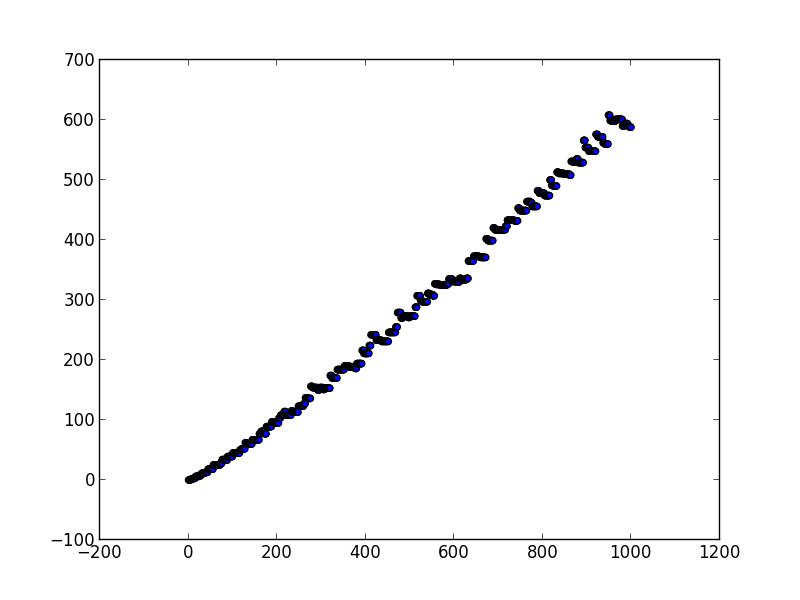
\includegraphics[width=0.4\linewidth]{TimeUntilStabilizeWithOnePeak}\label{fig:case1}} \qquad
\subfigure[Global earthquakes until stable. Horizontal axis is $n$ and vertical axis is the number of global earthquakes divided by $n$]{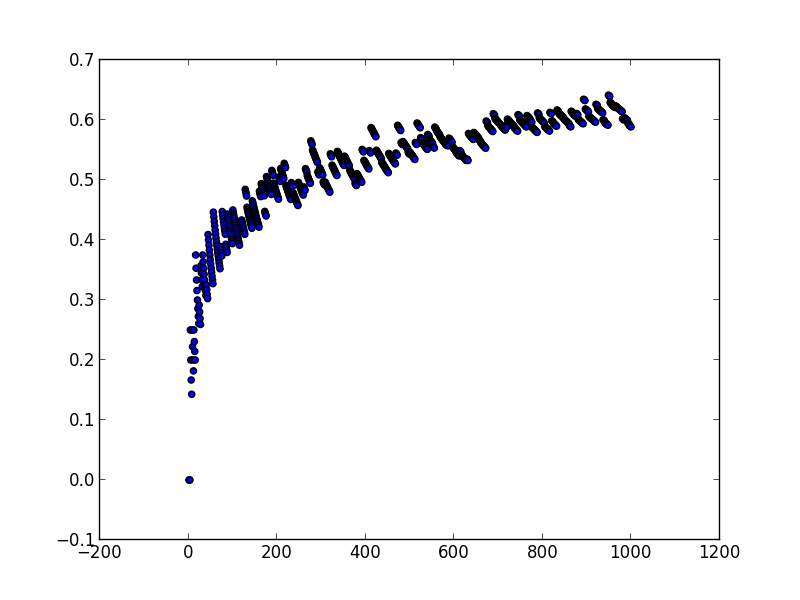
\includegraphics[width=0.4\linewidth]{Timeuntilstabledividedbyn}\label{fig:case2}}
\caption{Number of global earthquakes until stability}
\label{fig:growthofT}
\end{figure}
By looking at Figure~\ref{fig:growthofT} it seems that $T(n) = \Theta(n\log n)$. Our strategy to show a lower bound on $T(n)$ by giving a lower bound on $T'(n)$ seems to be the correct approach, since by experimental evidence (see Figure~\ref{fig:growthofT'}, we believe that $T'(n) = \Theta(n\log n)$.

\begin{figure}[!ht]
\centering
\subfigure[Local earthquakes of center until stable. Horizontal axis is $n$ and vertical axis is the number of local earthquakes]{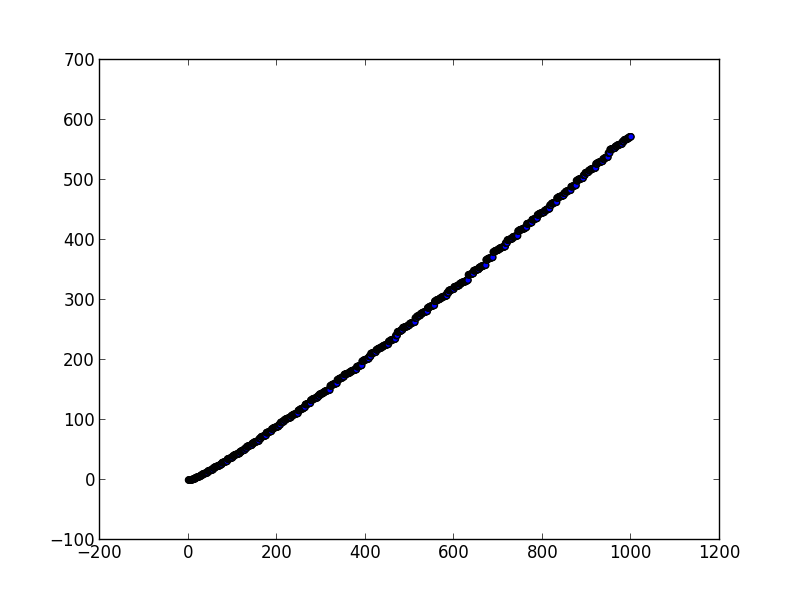
\includegraphics[width=0.4\linewidth]{centerearthquakes}\label{fig:case1}} \qquad
\subfigure[Local earthquakes of center until stable. Horizontal axis is $n$ and vertical axis is the number of local earthquakes divided by $n$]{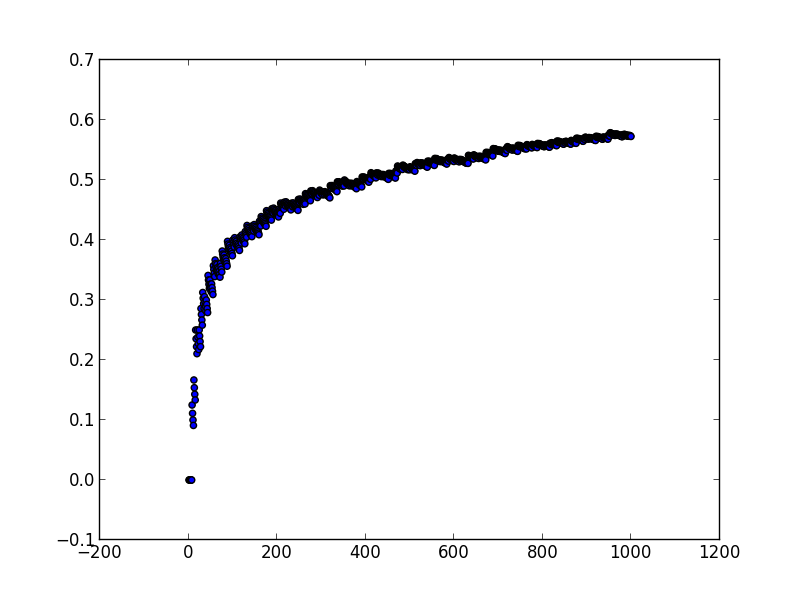
\includegraphics[width=0.4\linewidth]{centerearthquakesdividedbyn}\label{fig:case2}}
\caption{Number of local earthquakes in center until stability}
\label{fig:growthofT'}
\end{figure}



\section{Board Variants: $d$-Trees}
\label{Board Variants: d-Trees}
\emph{written by Perry Kleinhenz, edited by Fermi Ma and Erik Waingarten.}\\


\begin{definition}
A $d$-tree is a graph composed of a parent node connected by edges to $d-1$ unique children nodes.Those children each have $d-1$ unique children and so on.  
\end{definition}
We note that every node other than the original parent node has $d$ neighbors. In order to simplify our process we would like the graph to be regular and so we make the following definition. 
\begin{definition}
A joined $d$-tree is two $d$-trees connected at their parent nodes by an edge.
\end{definition}

We now define a coordinate system so that our method of proof can mirror that of the standard board case.
\begin{definition} We define a coordinate system for our joined $d$-trees, with the following rules:
\begin{enumerate}
	\item $(0,0)$ and $(1,0)$ are valid coordinates and refer to the two parent nodes.
	\item $(a,b)$ is a valid coordinate for $a<0$ if $0<b \leq (d-1)^{|a|}$
	\item $(a,b)$ is a valid coordinate for $a>1$ if $0<b \leq (d-1)^{|a-1|}$
\end{enumerate}
We define the set of all valid coordinates $G_d$ for a joined $d$-tree as 
\begin{equation}
G_d:= \{ (a,b) \in \mathbb{Z} \times \mathbb{Z} ; (a,b) \text{ obey the rules above}\}
\end{equation}
\end{definition}

In order to keep our notation compact we once again define a function that outputs the neighbors of a node
\begin{definition} 
We define the function $n: G_d \rightarrow G_d^d$ as 
\begin{equation*}
n(i,j) = \{ (x_1, y_1); (x_1 = i+1 \text{ or } x_1=i-1), \text{ and }(x_1, y_1) \in G_d\}
\end{equation*}
\end{definition}

We now formalize the board of poker chips. Note that this definition only differs from our initial definition in that the input value is a coordinate of a node in a joined $d$-tree rather than a coordinate in the integer lattice.
\begin{definition}
We define a $d$-board to be a map from the set of valid coordinates to the nonnegative integers, that is 
\begin{equation}
b:  G_d \rightarrow \mathbb{Z}_{\geq 0}
\end{equation}
We write $\mathcal{B}(d)$ to refer to the set of all $d$-boards.  
\end{definition}

Recalling that $n(s)$ refers to the neighbors of $s$ we define our earthquake operation in terms of $d$-boards.
\begin{definition}
An earthquake takes as an input an $d$-board and a node and outputs an $d$-board so we write $E: \mathcal{B}(d) \times G_d \rightarrow \mathcal{B}(d)$. If $s$ is the node input and $b(s)>d$ then 
\begin{align*}
E[b, s](s) = b(s)- d \\
E[b, s](t) = b(t) +1 
\end{align*}
for $t \in n(s)$. Otherwise $b(s)<d$ and $E[b,s]=b$ as the earthquake does not move any chips. We use the notation $E^r[b, \{s_k\}]$ to denote the application of $E$ to the $b$ $r$ times, to the sites $s_1, \ldots s_r$ respectively.
\end{definition}

Now that we have formalized the earthquake operator we can introduce a precise definition of stability of a board. 
\begin{definition}
We say that a $d$-board is stable if its values are strictly less than $n$.
\end{definition}
This is equivalent to saying all earthquakes have no effect on the board. We also make a precise definition for a finite board.
\begin{definition} 
We say that a $d$-board is finite if the total number of chips on it is finite. That is a $d$board $b$ is finite if the sum
\begin{equation}
C= \sum_{(i,j) \in G_d} b(i,j) 
\end{equation}
is finite. 
We denote the set of finite $d$-boards as $B(d)_F$.
\end{definition}

We will now show that any finite $d$-board will stabilize under earthquakes. Our method of proof will mirror the method used for the square lattice, without only minor changes.  Therefore we will proceed by shooing that if an earthquake changes the state of a $d$-board, then no sequence of earthquakes can transform the output $d$-board back into the original $d$-board. We will then give a bound on the maximum number of configurations a given $d$-board can be transformed into by earthquakes. Once again these together will show that all finite $d$-boards will stabilize.

We once again define a spread function 
\begin{definition}
 Let $\Psi: \mathcal{B}(d)_F \rightarrow \mathbb{Z}_{\geq 0}$ be the function
\begin{equation}
\Psi(f) = \sum_{(i,j) \in G_d} b(i,j) |i|^2
\end{equation}
Note that this is well defined for trees which contain a finite number of chips. 
\end{definition} 
We can once again think of this spread function as the sum of the number of chips on every node weighted by the taxi-cab distance from the node to the origin.

\begin{lemma}
If $E[b, s_1] \neq b$, then $E^r[b, \{s_k\}] \neq b$ for all $r>0$ and all sequences $\{s_k\}$ of length $r$ that begin with $s_1$. 
\end{lemma}

\begin{proof}
For ease of notation let $s=(s_1, s_2)$. We will show that if $E$ acts on a board nontrivially then $\Psi(E[b, s])$ will be strictly larger. That is  
\begin{equation}
E[b, s] \neq f \Rightarrow \Psi(E[b, s]) > \Psi(b)
\end{equation}


We can evaluate $\Psi(E[b, s]) - \Psi(b)$.
\begin{align}
\Psi(E[b, s])-\Psi(b) = \sum_{(i,j) \in G_d} E[b, s](i,j)|i|^2 - \sum_{(i,j) \in G_d} b(i,j)|i|^2 
\end{align}
We note that only $s$ and its neighbors are affected so our expression simplifies to
\begin{align*}
\Psi(E[b, s]) - \Psi(b) &= E[b, s](s) |s_1|^2 - b(s) |s_1|^2 + \sum_{(i,j) \in n(s)} (E[b,s](i,j) |i|^2 - b(i,j)|i|^2) \\
&= -d |s_1|^2 + \sum_{(i,j) \in n(s)} |i|^2
\end{align*}
We note that exactly $d-1$ of the neighbors of $s$ are a distance $|s_1 +1|$ from the origin and one of the neighbors of $s$ is a distance $(|s_1| - 1)$ from the origin.  A point to emphasize is that this is the only substantial way in which this proof differs from the similar proof for the square lattice. Our expression simplifies to 
\begin{align*}
&= -d |s_1|^2 + \sum_{(i,j) \in n(s)}-|i|^2 \\
&= - d|s_1|^2 + (d-1)(|s_1| +1)^2 +(|s_1| -1)^2 \\
&= d + (d-2)2|s_1| >0
\end{align*}
\end{proof}

\begin{lemma}
\label{finiteextensiontree}
Suppose $\sum_{x,y} f(x,y) = C$, and the first coordinate of all nodes which are nonzero are in $[i_{min}, i_{max}]$. Then $E^r[b, \{s_k\}]$ only contain chips within the range $[i_{min} - 2C, i_{max} + 2C]$ for all $r>0$ and all sequences $\{s_k\}$ of length $r$.
\end{lemma}

\begin{proof}
It is obvious that a board with $C$ chips on nodes with first coordinate $l<0$ will have a lower $i_{min}$ than a board with $S$ chips on level 0, and the analogous statement for $i_{max}$ holds as well. 

Now because chips cannot be transferred between two nodes whose first coordinate differs by more than 1, we know that $C$ chips on a single node with first coordinate $l<0$ will have an $i_{min}$ no lower than $l-2C$ as there must be at least one chip on every other level. 

If we take any other arrangement of $C$ chips, with $i_{min}=l$ but not all $C$ chips are on a single node. We know that $i_{min}$ for this board is bounded below by $l-2C$. In order to have an $i_{min}$ below this at some point in time it would be possible to have $C$ chips on the same node on level $l$. But this cannot occur because in order to move a chip to a node with a lower first coordinate, one chip must moved to a node with a higher first coordinate. Therefore $E^r[b, \{s_k\}]$ does not have a node with a nonzero number of chips on it with first coordinate less than $i_{min} -2C$.

An analogous argument shows that if $i_{max}$, both $GE_T^m(f)$ and $LE_T^m(f)$ do not have a node with a nonzero number of chips on it with first coordinate greater than $i_{max}+2C$.
\end{proof}

So now we are ready to prove the theorem that all finite boards will reach a stable state. 

\begin{proof}
(of Theorem~\ref{finitestability}) Suppose $b \in \mathcal{B}(d)_f$ is a finite board, so $\sum_{(i,j) \in G_n} b(i,j) = C$, and suppose all chips lie between levels  $[i_{min}, i_{max}]$. Then by Lemma ~\ref{finiteextensiontree}, we have that for all $r$ and sequence $\{s_k\}$ all chips in $E^r[b, \{s_k\}]$ will have first coordinate in $ [i_{min} -2C, i_{max} +2C]$.

We have restricted the size of the board to be finite, and the number of chips that can be placed on the board to be finite. 
Thus the total number of ways that the chips can be arranged on the board is finite. 
In particular there are fewer than $(i_{max} - i_{min}+1 + 4 C)$  and there are at most 
\begin{equation}
d^l,
\end{equation}
nodes at each level, where $l= \max(|i_{min}|, |i_{max}|)$. So there are at most 
\begin{equation}
N:=(i_{max} - i_{min}+1 + 4 C)d^l
\end{equation}
nodes that are potentially occupied. Therefore there are at most 
\begin{equation}
\binom{N+S-1}{N-1}
\end{equation}
possible boards $b \in \mathcal{B}(n)_f$ that satisfy this. We know that there are no cycles in the states, so there must be an $0 \leq N < \binom{N+S-1}{N-1}$ and some sequence $\{s_k\}$ such that $E^N[b, \{s_k\}] = E^{N+m}[b, \{s_k\}]$ for all $m \geq 0$.
\end{proof}


\section{Computing with Chips}
\label{Computing with Chips}

\emph{Written by Erik Waingarten, edited by Fermi Ma and Perry Kleinhenz.}

In this section, we show how we can compute different Boolean functions using the poker chip board and the earthquake operator.

A Boolean input is a number in $\{0,1\}$, and a Boolean function is a function that takes $k$ Boolean inputs and outputs a number in $\{0,1\}$. A simple Boolean function is the AND function that takes in 2 Boolean inputs, and returns a 1 if and only if both the input values are set to 1. Another Boolean function is the OR function, that takes in 2 Boolean inputs, and returns a 0 if and only if both input values are set to 0. If 0 is associated with ``false" and 1 is associated with '``true", then the AND function returns ``true" if both inputs are ``true", and the OR function returns ``true" if at least one input is true. More complicated Boolean functions can be made with more than 2 inputs and compositions of these inputs. Denoting an AND with $\vee$ an OR with $\wedge$, we can construct composite functions such as $b_1 \wedge (b_2 \vee b_3)$. 

Boolean circuits are formed by using wires that transmit 0's and 1's, and feeding them through various \emph{gates}. For example, a wire carrying a 0 and a wire carrying a 1 can be fed through an OR gate, which will ``output" a wire carrying a 1. In this section, we construct circuits using the poker chips board that use AND an OR gates. 

\subsection{Model of Computation}

Our model of computation is as follows: we assume a finite board with finitely many chips. The inputs are designated by each two squares, one apart one is the ``clock" square and other the bit square. Likewise, the outputs each have a ``clock" square and a bit square. The ``clock" squares are set the value 4 and the bit squres are set to 4 if they are 1 and 0 otherwise. A computation is done by a series of earthquakes, when an output has the clock square active, then the bit square is read, and that output bit is considered read. 

\subsection{Example}

A simple example is given by a board that computes the identity.

\[ \begin{array}{cccccc} 0 & 0 & 0 & 0 & 0 & 0 \\
				     4_c & 3 & 3 & 3 & 3 & 3_e \\
				     0 & 0 & 0 & 0 & 0 & 0 \\
				     i  & 3 & 3 & 3 & 3 & 3_o \\
				     0 & 0 & 0 & 0 & 0 & 0 \end{array} \]
Where the subscript $c$ indicates the clock, the subscript $e$ indicates the output clock square. $i$ indicates the bit square, and $o$ indicates the output bit. 

One can see that $e$ will become active after 5 earthquakes since it will take that many earthquakes for $c$ to reach $e$. Also, if $i$ is initially inactive, then $o$ will be inactive, and if $i$ is active, then $o$ will be active. Therefore, we can compute the identity. 

This circuit also shows how to make a ``wire" in the circuit. We will represent a wire as two parralel arrows, one containing the clock path and the other carrying the input. 

\subsection{Turner}

Turning is non trivial, we must guarantee that we can turn a signal and align the timinings of the inputs and outputs in the clock so that they have the same distance. this is a counter-clockwise turn where $c$ denotes the clock, $i$ is the input bit, then $e$ is the output clock and $o$ is the output bit.

\[ \begin{array}{cccccc} 0 & 0 & e & 0 & o \\
				     0 & 3 & 2 & 0 & 3 \\
			            0 & 2 & 3 & 0 & 3 \\
				    0 & 3 & 2 & 0 & 3 \\
				    0 & 2 & 3 & 0 & 3 \\
				    c & 3 & 3 & 0 & 3 \\
				    0 & 0 & 0 & 0 & 3 \\
				    i & 3 & 3 & 3 & 3 \end{array} \]	
Since the clock snakes along the path while $i$ takes the shorter path. 
Likewise, we can perform a clockwise path by making $i$ snakes while the clock takes a straight path. 

\subsection{Synchronize}

We can synchronize the inputs so that the input signal waits for the clock to arrive. This can be simply done with the following board configuration:
\[ \begin{array}{cccccccc} c & 3 & 3 & 3 & 3 & 3 & 3 & 0 \\
					 0 & 0 & 0 & 0 & 3 & 0 & 3 & 0 \\
					 i  & 3 & 3 & 3 & 1 & 3 & 3 & 3 \\
					 0 & 0 & 0 & 0 & 3 & 0 & 0 & 3 \\
					 0 & 0 & 0 & 0 & o & 0 & e & 3 \end{array} \]
Note that the path from $i$ to $o$ is 6 units long, while the path from clock is 12 unit long. $i$ waits for the clock since it needs the signal from $c$ from two sides to activate the 1 in the path from $i$ to $o$.

The fact that we have a synchronizer means that the model of computation is equivalent to one where there is only one clock for all input bits. 

\subsection{Boolean circuits}

Now we can show how to compute some basic boolean functions and since we have turns and synchronizers, we can assume that we have synchronized the inputs already. The following can compute the AND of two inputs. 

\[ \begin{array}{cccccccc}    &    & c_1&   &  i_1 &     &  \\
					   &    & 3   & 2 &  3    &    &  \\
					   &    &    & 3 &    & 3 & c_2 \\
					o & 3 & 3 & 2 & 3 & 2 & 	    \\
					   &    &    &    &    & 3 & i_2 \end{array} \]
Where we can make the $c_1$ and $c_2$ snake around before hand to guarantee that they are synchronized, and then we can make $c_1$ snake around so that it becomes the clock of the output. So in this case, $o = i_1$ AND $i_2$.

Similarly, we can compute the OR of two circuits with a very simple modification:
\[ \begin{array}{cccccccc}    &    & c_1&   &  i_1 &     &  \\
					   &    & 3   & 2 &  3    &    &  \\
					   &    &    & 3 &    & 3 & c_2 \\
					o & 3 & 3 & 3 & 3 & 2 & 	    \\
					   &    &    &    &    & 3 & i_2 \end{array} \]
And we can do a similar set up to synchronize the clocks. 

So currently, we can compute any boolean circuit which can be drawn in a planar graph with only ANDs and ORs. So the question is whether we can compute the NOT? We argue that this is not possible. 

\begin{theorem}
There does not exists any board configuration which computes the NOT operator in the above model of computation.
\end{theorem}

\begin{proof}
Suppose we have a board configuration $B$ with input squares $c$, $i$ and output squares $e, o$ that computes the NOT function. Then we can make another board $B'$ that synchronizes the final clock with the input so that we do not need to worry about timing of the clock. That is, we can guarantee that if $o$ is active, then $o$ is active at the same time $e$ is active.

Now lets make $B'$ an infinite board by putting 0s on the sides. So we have a finite board with finitely many chips. Let $S_{c_0i_0}$ be the set of squares which were active (had an earthquake affect them) during the execution of $B$ with the input value $i = i_0$ and $c = c_0$. 

The first claim to make is that $S_{c_0i_0} \subset S_{c_1i_1}$ if $c_0 \leq c_1$ and $i_0 \leq i_1$. This is clearly true since the order of redistribution does not matter. In fact, we can do the earthquakes by first doing the earthquakes on $c$ and $i$ until the value decreases past $c_0$ and $i_0$, then simulate the computation of $c = c_0$ and $i = i_0$ with local earthquakes.

However, this arises in a contradiction, since $o \in S_{10}$ but $o \notin S_{11}$. Therefore, computing NOT with a board is not possible.
\end{proof}

What does this mean? Well, in particular, it means that we cannot do much. In particular, we can't add, since $x + 1$ will act as the NOT operator on the lowest order bit. We can only compute boolean circuits in planar graphs. 


\end{document}
